
%%%%%%%%% MASTER -- compiles the 4 sections

\documentclass[11pt,letterpaper]{article}

\usepackage{graphicx}
\usepackage{verbatim}
\usepackage{listings}
\usepackage{amssymb,amsmath}

%%%%%%%%%%%%%%%%%%%%%%%%%%%%%%%%%%%%%%%%%%%%%%%%%%%%%%%%%%%%%%%%%%%%%%%%%
\pagestyle{plain}                                                      %%
%%%%%%%%%% EXACT 1in MARGINS %%%%%%%                                   %%
\setlength{\textwidth}{6.5in}     %%                                   %%
\setlength{\oddsidemargin}{0in}   %% (It is recommended that you       %%
\setlength{\evensidemargin}{0in}  %%  not change these parameters,     %%
\setlength{\textheight}{8.5in}    %%  at the risk of having your       %%
\setlength{\topmargin}{0in}       %%  proposal dismissed on the basis  %%
\setlength{\headheight}{0in}      %%  of incorrect formatting!!!)      %%
\setlength{\headsep}{0in}         %%                                   %%
\setlength{\footskip}{.5in}       %%                                   %%
%%%%%%%%%%%%%%%%%%%%%%%%%%%%%%%%%%%%                                   %%
\newcommand{\required}[1]{\section*{\hfil #1\hfil}}                    %%
\renewcommand{\refname}{\hfil References Cited\hfil}                   %%
\bibliographystyle{plain}                                              %%
%%%%%%%%%%%%%%%%%%%%%%%%%%%%%%%%%%%%%%%%%%%%%%%%%%%%%%%%%%%%%%%%%%%%%%%%%

%PUT YOUR MACROS HERE

\date{Due April 30th, 2012}
\title{CS 395 Homework 9}

\author{Colby Blair}

\begin{document}
\maketitle

\begin{center}

Grade: \_\_\_\_\_\_\_\_\_\_\_\_\_\_\_\_\_\_\_\_
\end{center}

\thispagestyle{empty}

\pagebreak


\section*{PROBLEMS}

\subsection*{1.}
The \textbf{maximum} number of elements in a heap happens when the heap is entirely filled out on the 
lowest level, meaning it is entirely filled out. This can be found with the equation $ 2^{k + 1} - 1 $.

The \textbf{minimum} number of elements in a heap happens when the lowest level only has one node.
The levels above the last level are complete, so the minimum can be found with the equation 
$2^{(k-1) + 1} - 1 + 1$, $ = 2^k$.


\subsection*{2.}
The tree is \textbf{not a max heap}, as it violates the max heap property with the node value 6:

\begin{figure}[!h]

	\begin{center}
	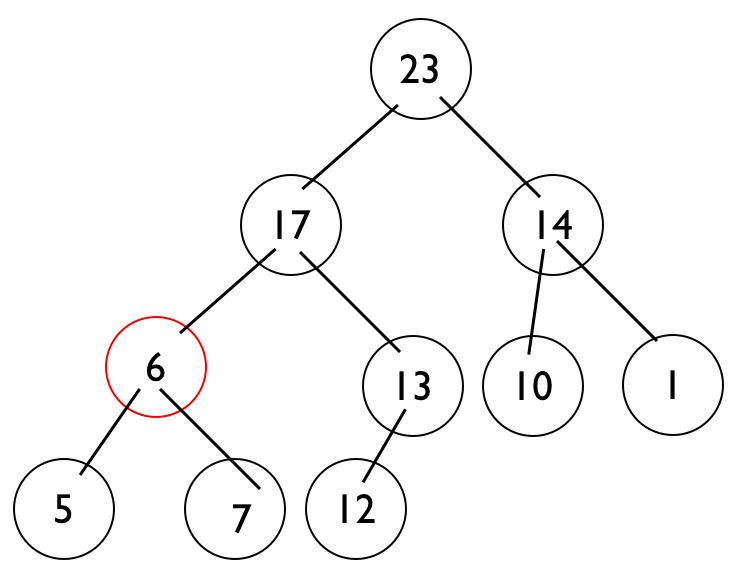
\includegraphics[width=110mm]{images/6_6_tree.png}
	\end{center}

\caption{Heap for the array \{23,17,14,6,13,10,1,5,7,12\} }
\end{figure}


\subsection*{3.}
Consider the operations on heap $ \{27,17,3,16,13,10,1,5,7,12,4,8,9,0\} $ for MAX\_HEAPIFY:

\begin{figure}[!h]

	\begin{center}
	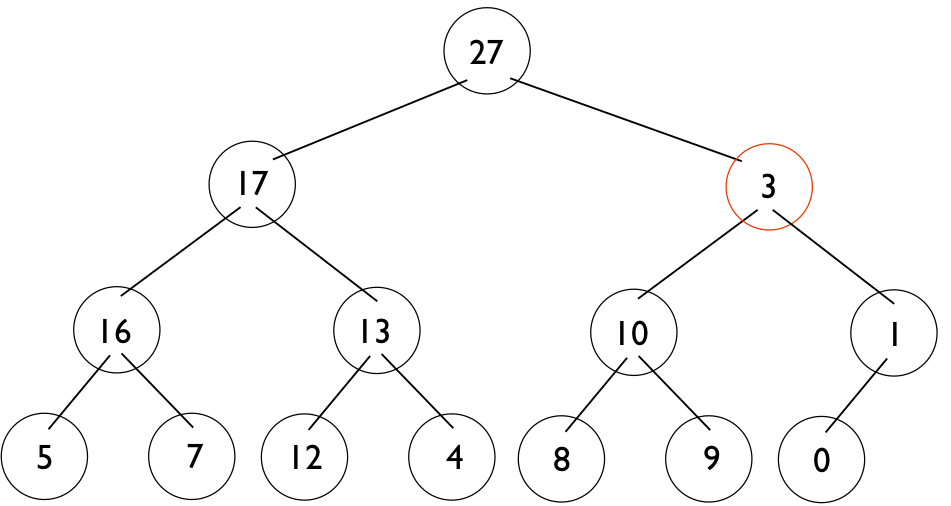
\includegraphics[width=80mm]{images/6_2_1_1_tree.png}
	\end{center}

\caption{Step 1 }
\end{figure}

\begin{figure}[!h]

	\begin{center}
	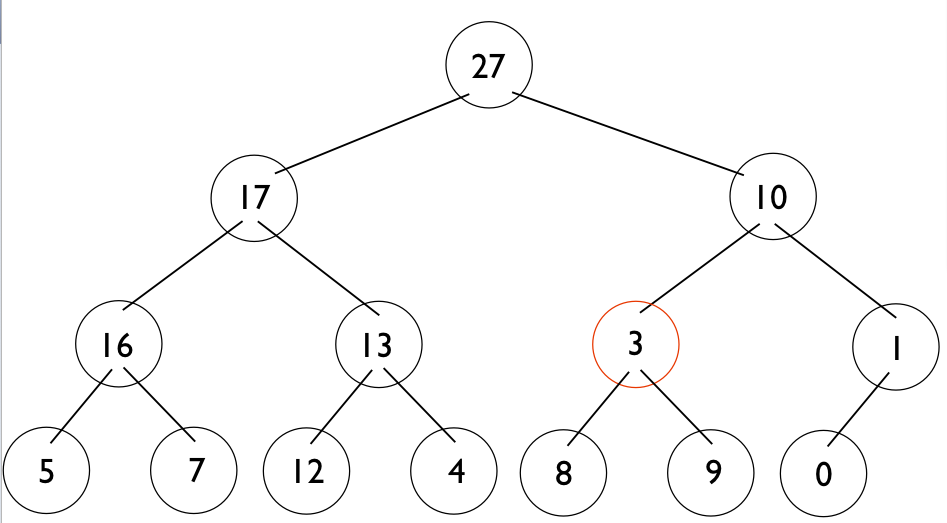
\includegraphics[width=80mm]{images/6_2_1_2_tree.png}
	\end{center}

\caption{Step 2 }
\end{figure}

\pagebreak

\begin{figure}[!h]

	\begin{center}
	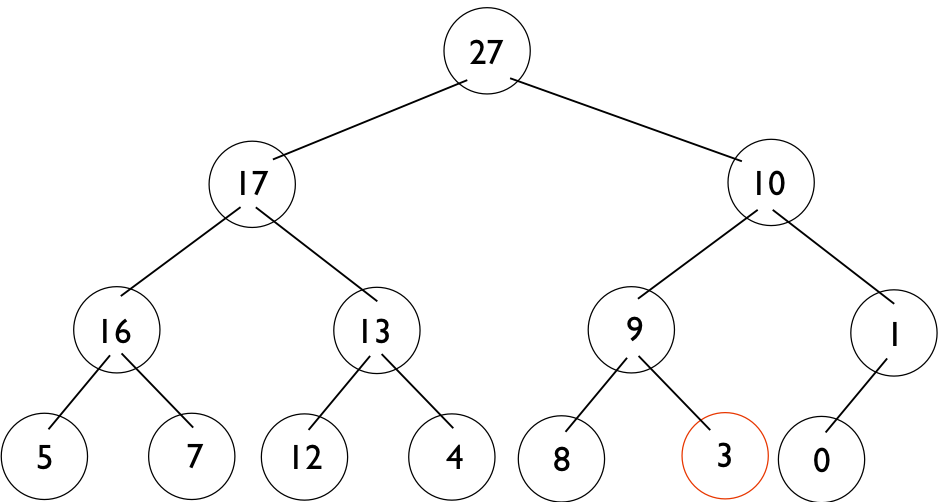
\includegraphics[width=80mm]{images/6_2_1_3_tree.png}
	\end{center}

\caption{Step 3 }
\end{figure}


\pagebreak


\subsection*{4.}
Consider the operations on heap $ \{5, 3, 17, 10, 84, 19, 6, 22, 9\} $ for BUILD\_MAX\_HEAP:

\begin{figure}[!h]

	\begin{center}
	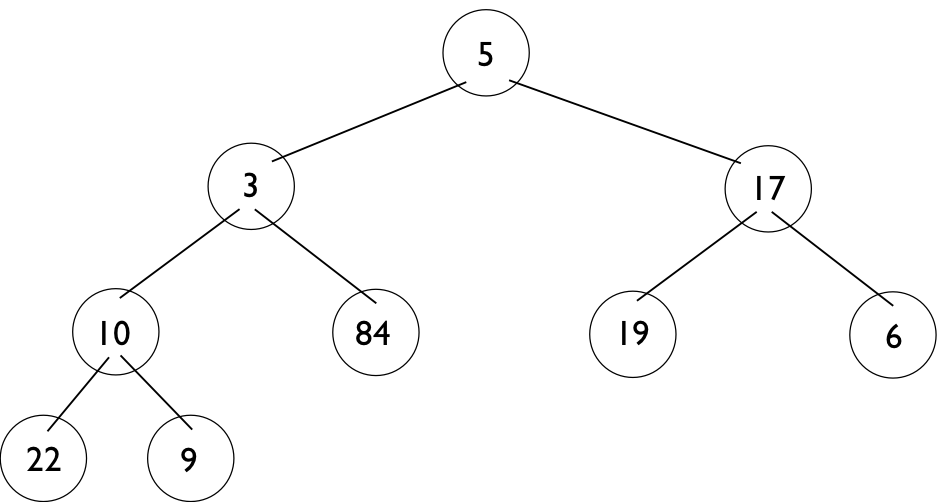
\includegraphics[width=80mm]{images/6_3_1_1_tree.png}
	\end{center}

\caption{Step 1 }
\end{figure}

\begin{figure}[!h]

	\begin{center}
	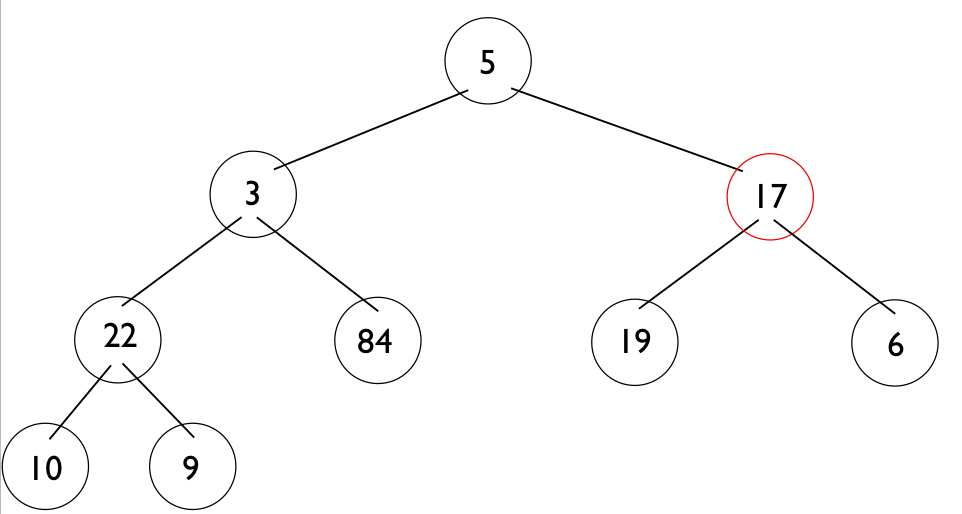
\includegraphics[width=80mm]{images/6_3_1_2_tree.png}
	\end{center}

\caption{Step 2 }
\end{figure}

\pagebreak

\begin{figure}[!h]

	\begin{center}
	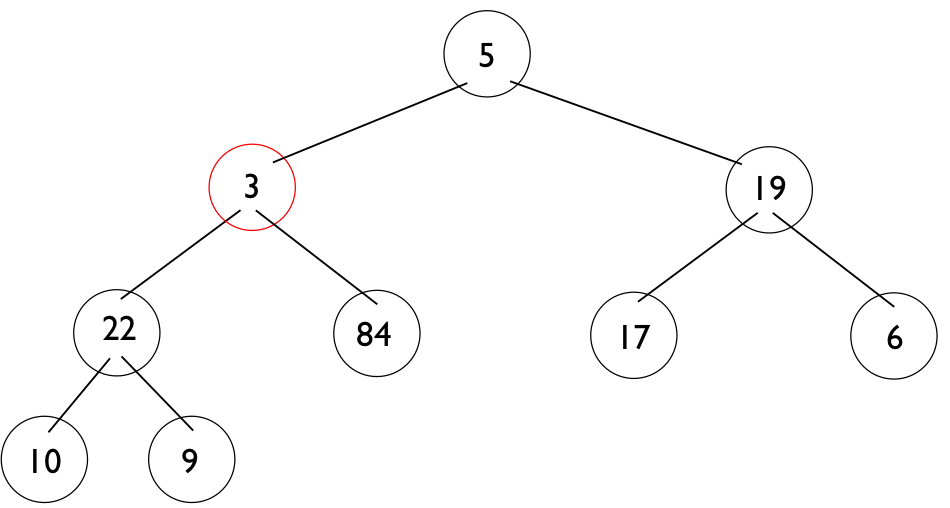
\includegraphics[width=80mm]{images/6_3_1_3_tree.png}
	\end{center}

\caption{Step 3 }
\end{figure}

\begin{figure}[!h]

	\begin{center}
	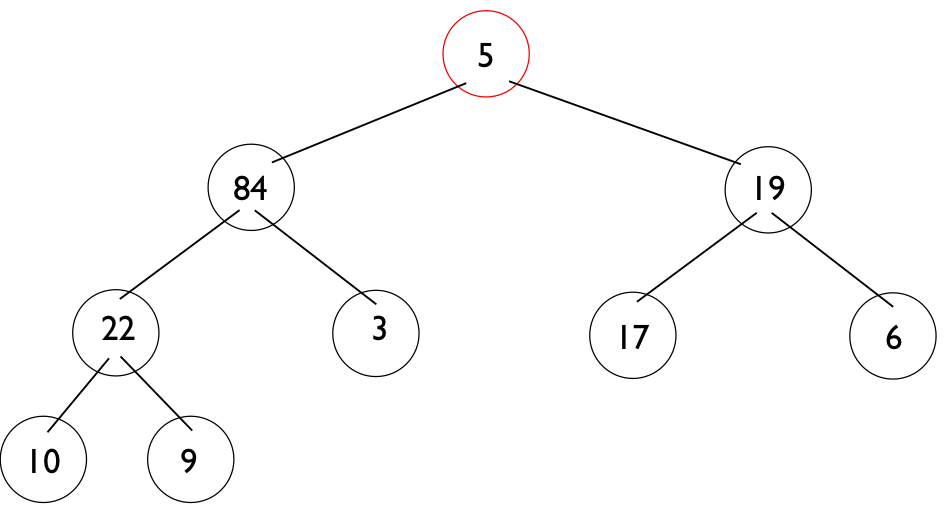
\includegraphics[width=80mm]{images/6_3_1_4_tree.png}
	\end{center}

\caption{Step 4 }
\end{figure}

\pagebreak

\begin{figure}[!h]

	\begin{center}
	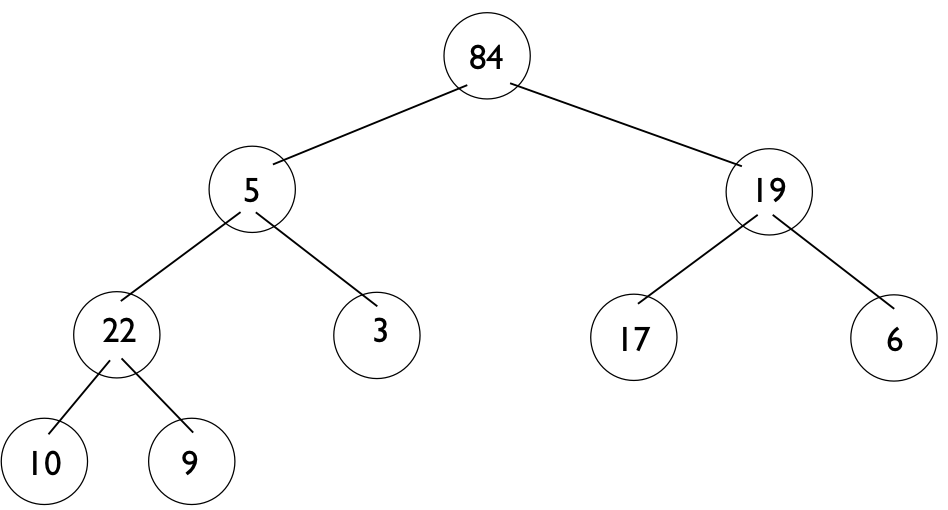
\includegraphics[width=80mm]{images/6_3_1_5_tree.png}
	\end{center}

\caption{Step 5 }
\end{figure}

\begin{figure}[!h]

	\begin{center}
	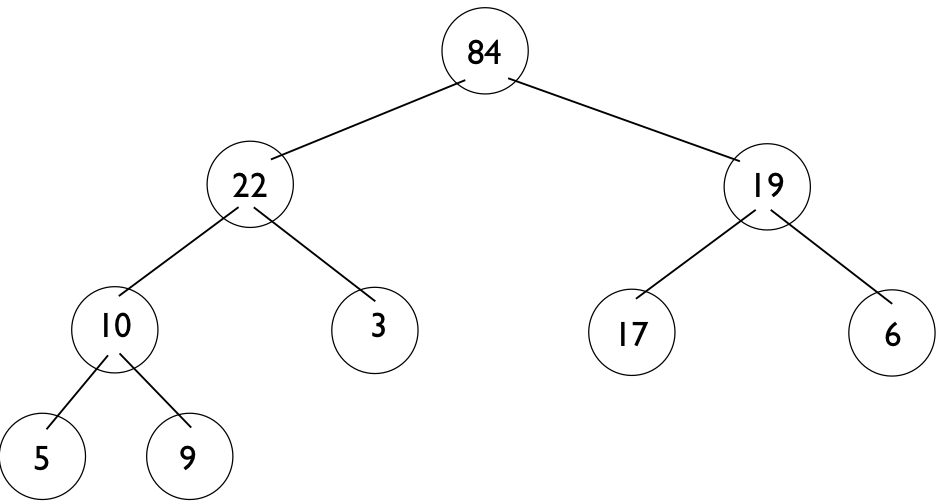
\includegraphics[width=80mm]{images/6_3_1_6_tree.png}
	\end{center}

\caption{Step 6 }
\end{figure}


\pagebreak


\subsection*{5.}
Consider the operations on heap $ \{5,13,2,25,7,17,20,8,4\} $ for BUILD\_MAX\_HEAP:

\begin{figure}[!ht]

	\begin{center}
	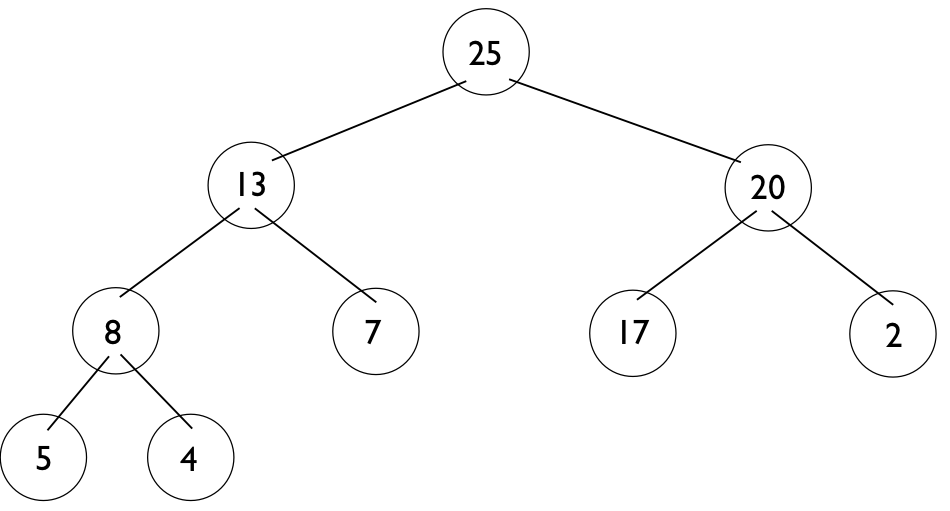
\includegraphics[width=80mm]{images/6_4_1_1_tree.png}
	\end{center}

\caption{Step 1 }
\end{figure}

\begin{figure}[!ht]

	\begin{center}
	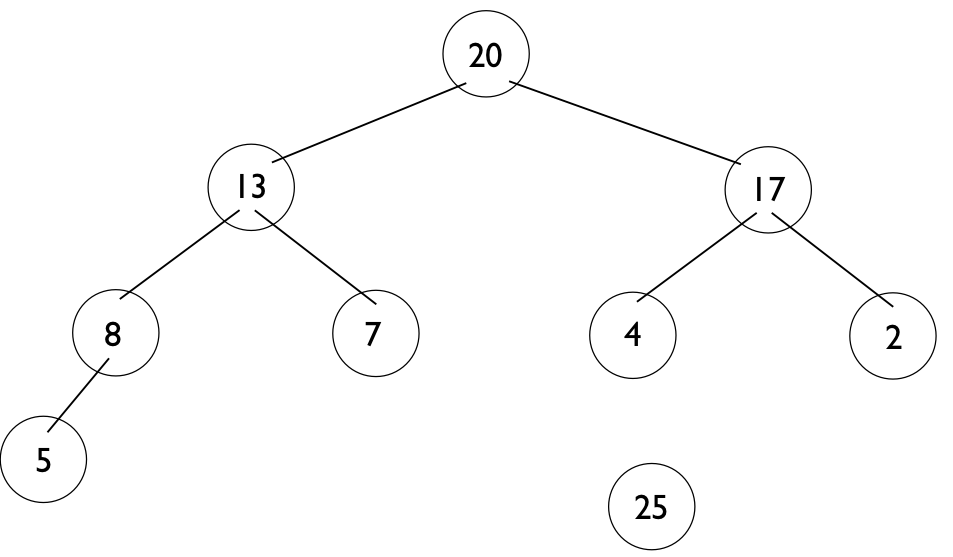
\includegraphics[width=80mm]{images/6_4_1_2_tree.png}
	\end{center}

\caption{Step 2 }
\end{figure}

\pagebreak

\begin{figure}[!ht]

	\begin{center}
	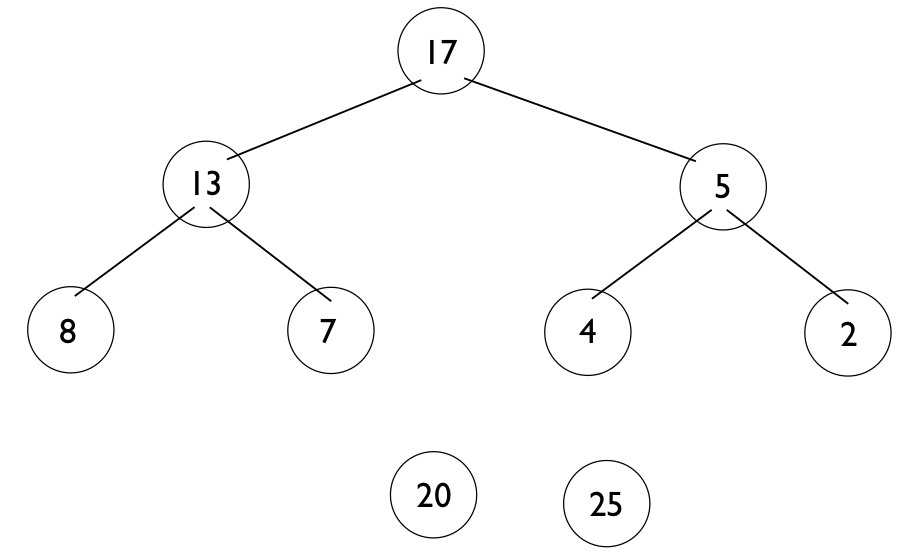
\includegraphics[width=80mm]{images/6_4_1_3_tree.png}
	\end{center}

\caption{Step 3 }
\end{figure}

\begin{figure}[!ht]

	\begin{center}
	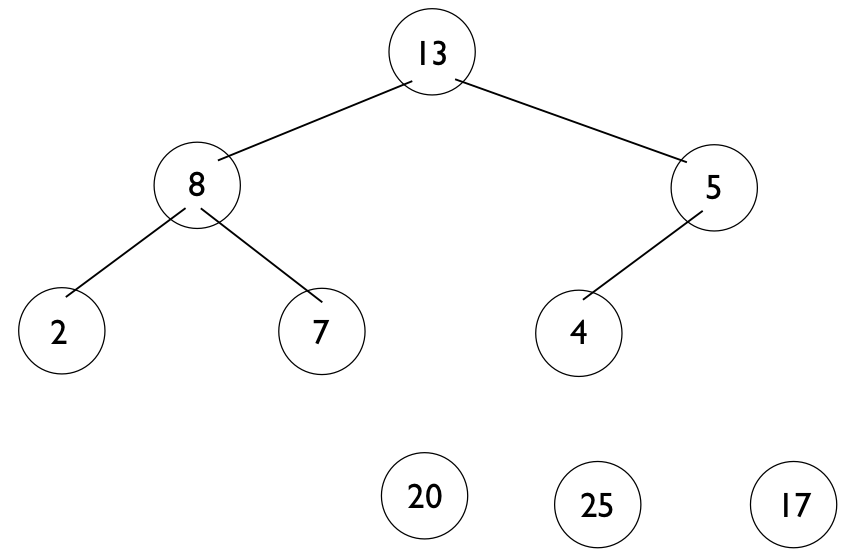
\includegraphics[width=80mm]{images/6_4_1_4_tree.png}
	\end{center}

\caption{Step 4 }
\end{figure}

\pagebreak

\begin{figure}[!ht]

	\begin{center}
	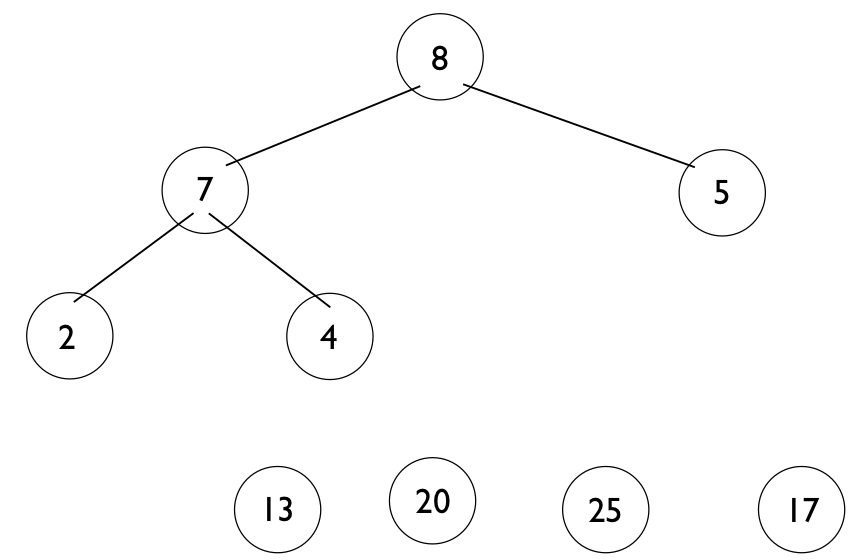
\includegraphics[width=80mm]{images/6_4_1_5_tree.png}
	\end{center}

\caption{Step 5 }
\end{figure}

\begin{figure}[!ht]

	\begin{center}
	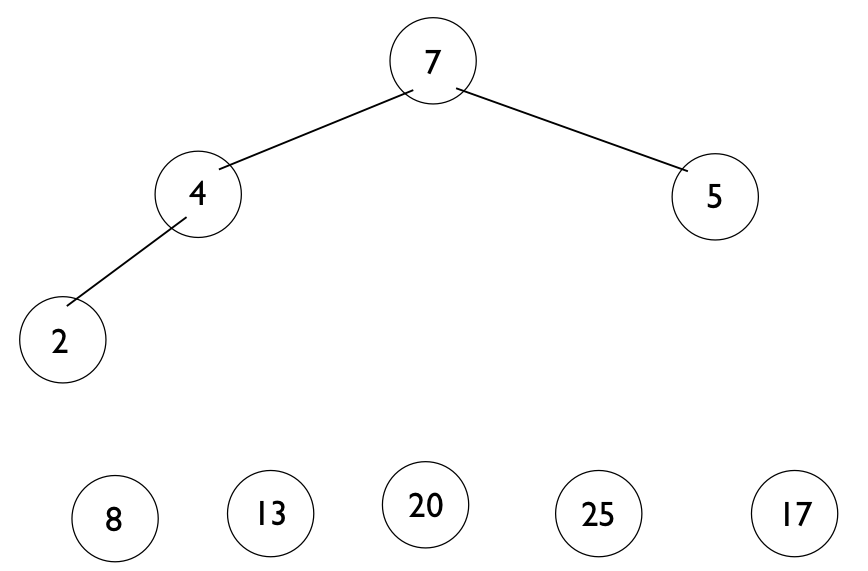
\includegraphics[width=80mm]{images/6_4_1_6_tree.png}
	\end{center}

\caption{Step 6 }
\end{figure}


\pagebreak


\subsection*{6.}
Consider the operations on heap \{15,13,9,5,12,8,7,4,0,6,2,1\} for HEAP\_EXTRACT\_MAX:

\begin{figure}[!ht]

	\begin{center}
	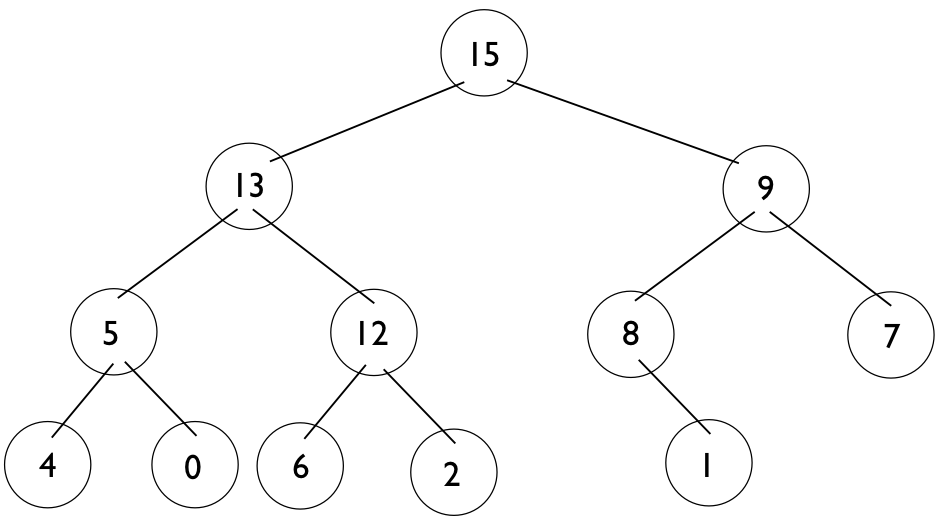
\includegraphics[width=80mm]{images/6_5_1_1_tree.png}
	\end{center}

\caption{Step 1 }
\end{figure}

\begin{figure}[!ht]

	\begin{center}
	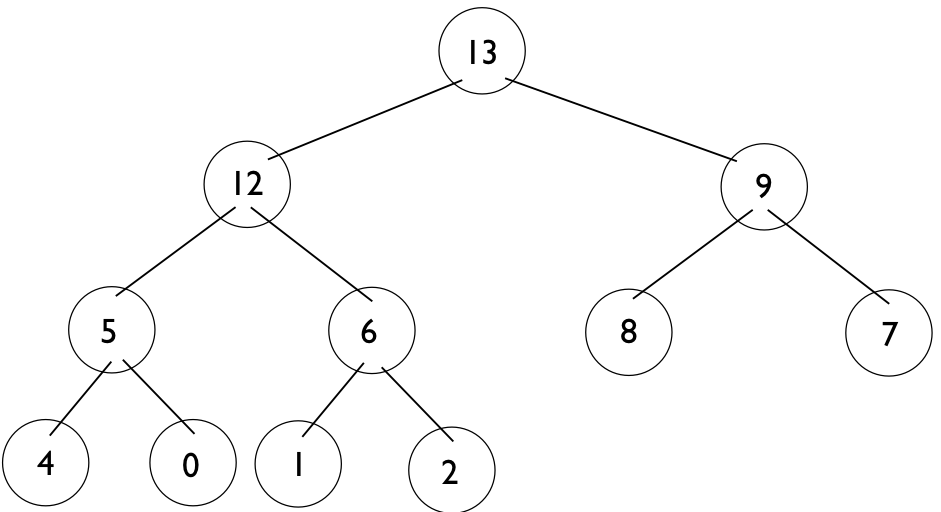
\includegraphics[width=80mm]{images/6_5_1_2_tree.png}
	\end{center}

\caption{Step 2 }
\end{figure}

\pagebreak

\begin{figure}[!ht]

	\begin{center}
	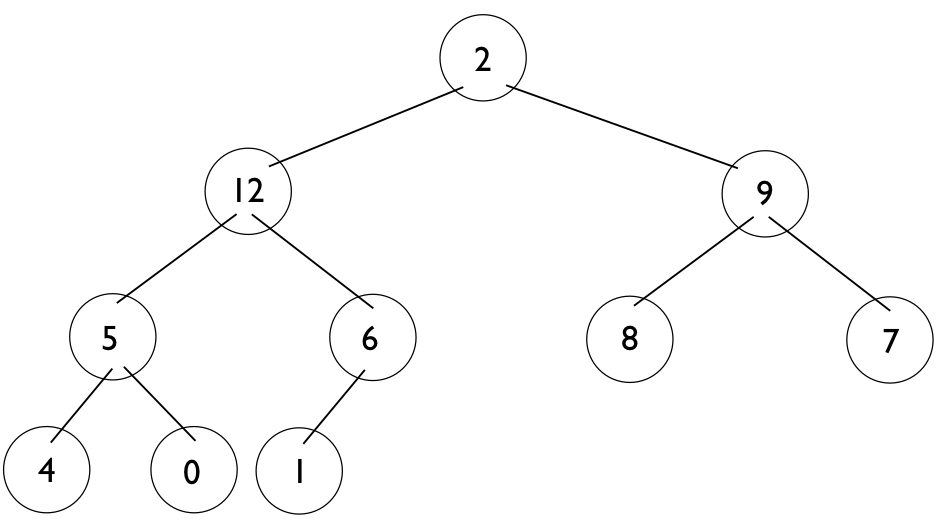
\includegraphics[width=80mm]{images/6_5_1_3_tree.png}
	\end{center}

\caption{Step 3 }
\end{figure}

\begin{figure}[!ht]

	\begin{center}
	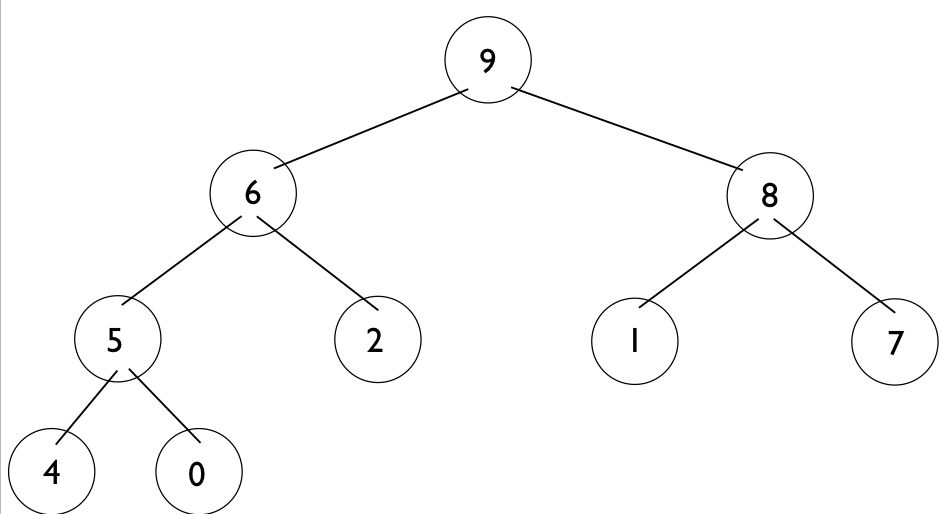
\includegraphics[width=80mm]{images/6_5_1_4_tree.png}
	\end{center}

\caption{Step 4 }
\end{figure}

\pagebreak

\begin{figure}[!ht]

	\begin{center}
	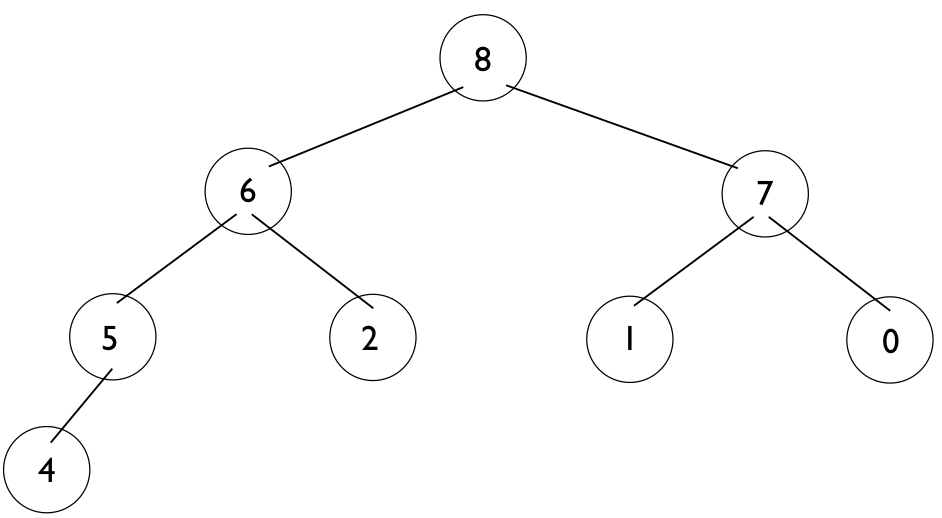
\includegraphics[width=80mm]{images/6_5_1_5_tree.png}
	\end{center}

\caption{Step 5 }
\end{figure}

\begin{figure}[!ht]

	\begin{center}
	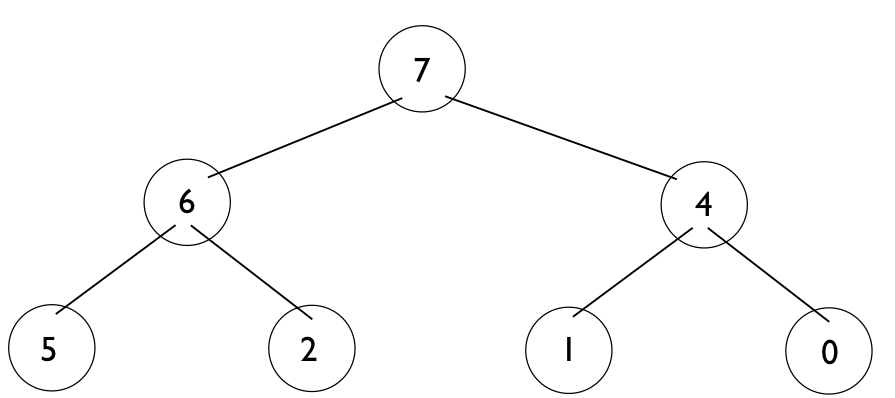
\includegraphics[width=80mm]{images/6_5_1_6_tree.png}
	\end{center}

\caption{Step 6 }
\end{figure}

\pagebreak

\begin{figure}[!ht]

	\begin{center}
	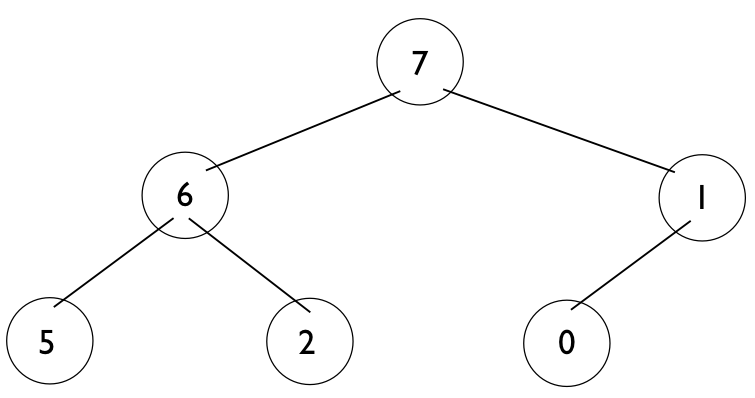
\includegraphics[width=80mm]{images/6_5_1_7_tree.png}
	\end{center}

\caption{Step 7 }
\end{figure}

\begin{figure}[!ht]

	\begin{center}
	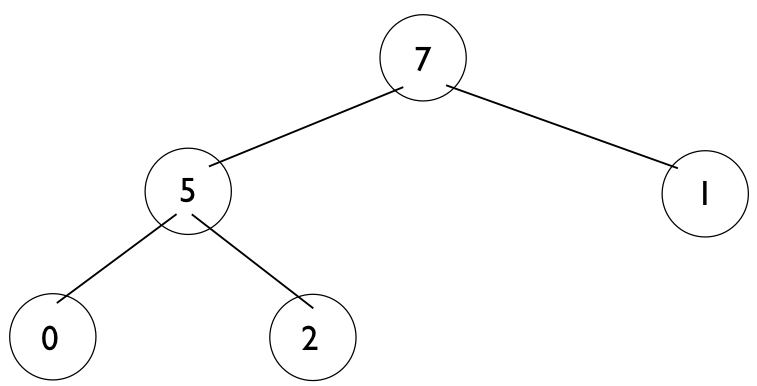
\includegraphics[width=80mm]{images/6_5_1_8_tree.png}
	\end{center}

\caption{Step 8 }
\end{figure}

\pagebreak

\begin{figure}[!ht]

	\begin{center}
	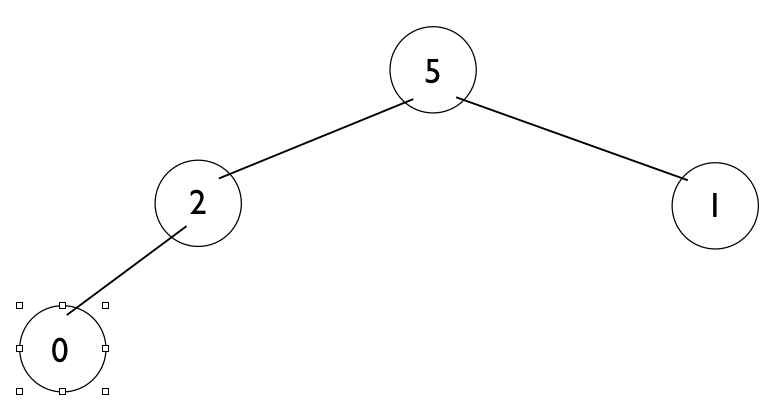
\includegraphics[width=80mm]{images/6_5_1_9_tree.png}
	\end{center}

\caption{Step 9 }
\end{figure}

\begin{figure}[!ht]

	\begin{center}
	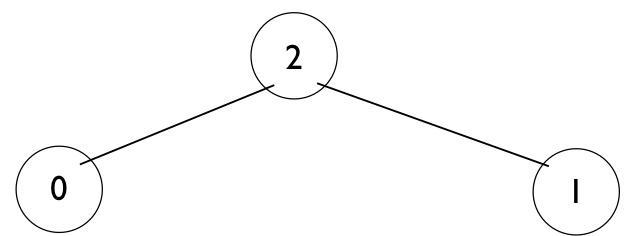
\includegraphics[width=80mm]{images/6_5_1_10_tree.png}
	\end{center}

\caption{Step 10 }
\end{figure}

\pagebreak

\begin{figure}[!ht]

	\begin{center}
	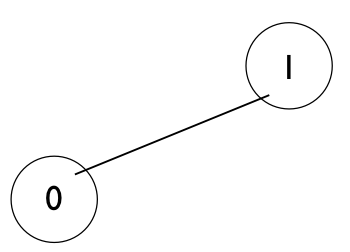
\includegraphics[width=80mm]{images/6_5_1_11_tree.png}
	\end{center}

\caption{Step 11 }
\end{figure}

\begin{figure}[!ht]

	\begin{center}
	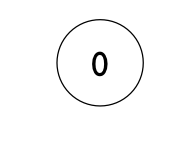
\includegraphics[width=80mm]{images/6_5_1_12_tree.png}
	\end{center}

\caption{Step 12 }
\end{figure}


\pagebreak

\subsection*{7.}
Consider the operations on heap \{15,13,9,5,12,8,7,4,0,6,2,1\} for MAX\_HEAP\_INSERT:

\begin{figure}[!ht]

	\begin{center}
	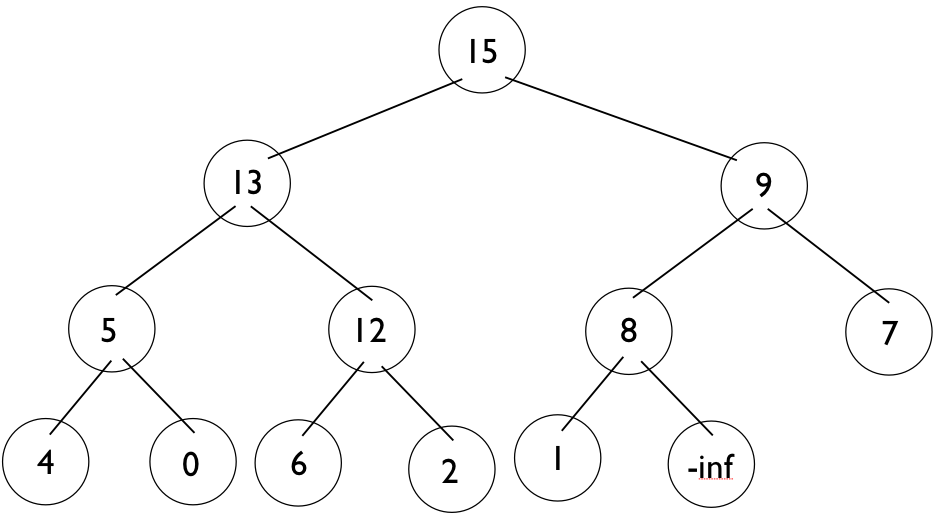
\includegraphics[width=80mm]{images/6_5_2_1_tree.png}
	\end{center}

\caption{Step 1 }
\end{figure}

\begin{figure}[!ht]

	\begin{center}
	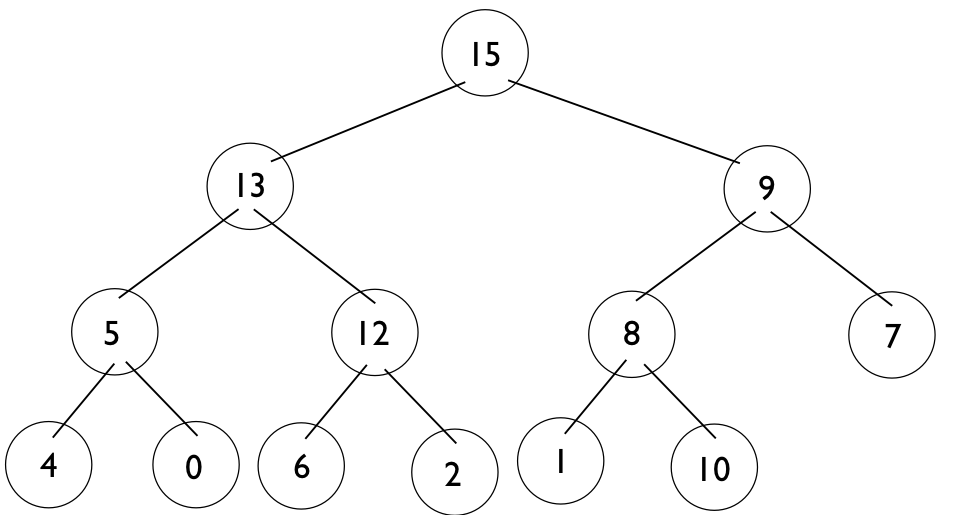
\includegraphics[width=80mm]{images/6_5_2_2_tree.png}
	\end{center}

\caption{Step 2 }
\end{figure}

\pagebreak

\begin{figure}[!ht]

	\begin{center}
	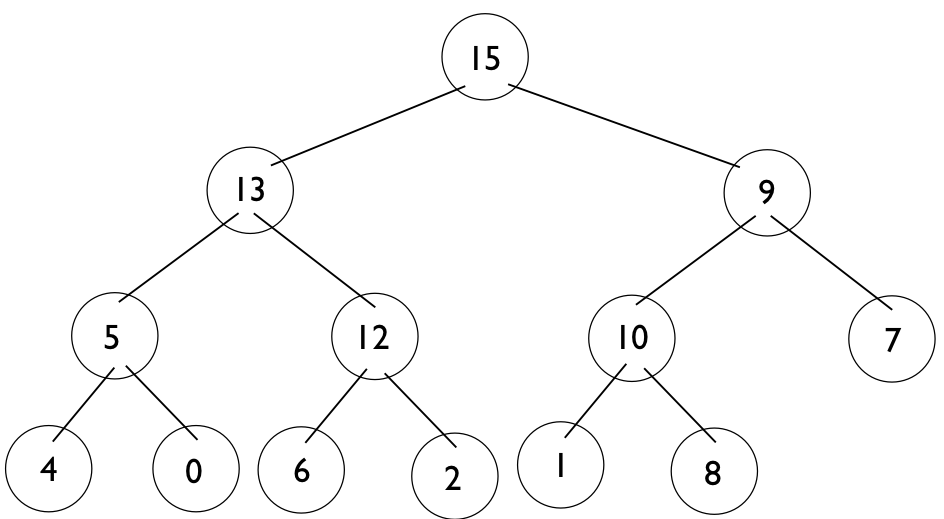
\includegraphics[width=80mm]{images/6_5_2_3_tree.png}
	\end{center}

\caption{Step 3 }
\end{figure}

\begin{figure}[!ht]

	\begin{center}
	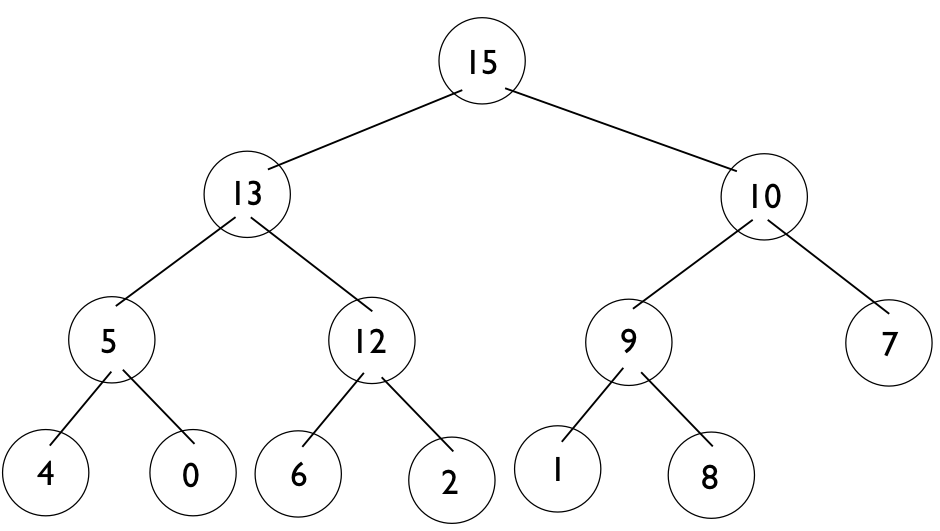
\includegraphics[width=80mm]{images/6_5_2_4_tree.png}
	\end{center}

\caption{Step 4 }
\end{figure}


\end{document}